\documentclass[a4paper]{sbgames}
%\usepackage[scaled=.92]{helvet}
\usepackage{times}
\usepackage{graphicx}

%% use this for zero \parindent and non-zero \parskip, intelligently.
\usepackage{parskip}

%% the 'caption' package provides a nicer-looking replacement
\usepackage[labelfont=bf,textfont=it]{caption}

\usepackage{url}

\usepackage{xcolor}
\newcommand{\toDo}[1]{\textcolor{red}{#1}}

\newcommand{\insertPicture}[1]{\textcolor{green}{#1}:
	\begin{figure}[h]
		\centering
		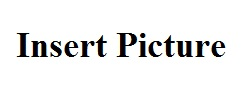
\includegraphics[width=150pt]{defaultPicture.jpg}
		\caption{\label{Label}Proper picture.}
	\end{figure}
	\\
	}

\title{Evolving Finite-State Machines Controllers for the Simulated Car Racing Championship}

\author{Bruno H. F. Macedo\\Gabriel F. P. Araujo\\
		\and Gabriel S. Silva\\Matheus C. Crestani\\\textit{University of Bras\'{i}lia}
		\and Yuri B. Galli\\ Guilherme N. Ramos\\
}

\contactinfo{gnramos@unb.br}

\keywords{finite-state machine, computer games, machine learning, genetic algorithm, TORCS, simulated car racing}
\newcommand{\gnramos}[1]{\textcolor{red}{#1}}%
\begin{document}

	\maketitle

	\begin{abstract}
		Autonomous vehicles have many practical applications, but the development of such controllers is a difficult task. This work presents a finite state-machine model with evolved parameters as a suitable solution for a self-driving car, and the comparison of two different configurations in The Open Racing Car Simulator. This approach enables a clear division of behaviors in states, providing an easy way to test different configurations and simplifying the search for better controllers by allowing changes in selected states. A 5-state and a 3-state drivers were evolved through genetic algorithm and compared to each other and to AUTOPIA, the current state of the art controller for the Simulated Car Racing Championship. Results showed that the proposed model has potential for racing, even surpassing one of AUTOPIA's marks, and provide insights on developing and configuring .
	\end{abstract}

	\keywordlist
	\contactlist

	\section{Introduction}\label{sec:1}

Automation of day to day tasks is an endeavor that has moved a large amount of scientific resources in the recent history~\cite{INDUS,APPLI}. One of the more desirable goals is the advent of self-driving cars, which should drive safely and efficiently, within traffic laws~\cite{SAFE,AUTOM}, bringing hope to current issues of traffic in urban roads by aiming at shorter response times, better fuel consumption, and lower levels of pollution. Such drivers, however, face several difficult challenges such as perception, navigation and control~\cite{6179503}.

Another critical issue is driver development, since testing is a frequent task and real driving systems are expensive. Creating and testing solutions can be aided by realistic car racing games which can closely simulate the roads, other vehicles, and their complex interactions~\cite{caldeira2013torcs}. Games also present a well defined environment which may be used not only for applications of machine learning results, such as neuroevolution~\cite{stanley_real-time_2005,} or human pose recognition~\cite{Shotton:2011}, but also for comparing AI solutions for specific problems such as path planning~\cite{deFreitas:2012}, controlling human non-playable character~\cite{simon2008}, car racing~\cite{2009}, among others.

The Open Racing Car Simulator (TORCS) is a modern, modular, highly-portable multi-player, multi-agent car simulator~\cite{SIMUTORCS}, one of the most advanced racing games available, and frequently used as a platform for comparing driver solutions in the Simulated Car Racing Championship (SCR)~\cite{2009,Loiacono:2012:LEA:2212908.2212953}. This paper uses a finite-state machine (FSM) controller to exploit the advantages of a divide-and-conquer approach by considering the task's various situations as distinct states (racing, getting unstuck, getting back on track, etc.).

FSM is a well-known mathematical model with widespread applications such as controlling air conditioning systems~\cite{BERNARD}, highway surveillance systems~\cite{DOHYUN}, and even simulated car racing~\cite{DIEGO}. Such solutions are implemented as software and configured according to a specified set of parameters, and defining the best possible configuration is usually a huge combinatorial problem for which exhaustive systematic searches become unfeasible. Thus, several machine learning approaches have been applied to it (heuristic algorithms~\cite{MrRacer}, modular fuzzy architectures~\cite{AUTOPIA}, \gnramos{inserir mais exemplos *com* referencias}, among others). One of the most successful optimization methods is Genetic Algorithm (GA), which is has been applied to a myriad of problems such as non-linear systems identification~\cite{GACTRL}, biomedicine prosthesis development~\cite{GABIO}, agent behavior forecasting~\cite{GAECO}, improving classifiers~\cite{pedrycz_genetic_2005}, and others.

This work uses a GA for searching for optimal parameter settings for the proposed FSM based driver, using TORCS as test bed. The rest of this paper is structured as follows: Section~\ref{sec:2} introduces the TORCS/SCR, finite-state machines, and Genetic Algorithms concepts involved; Section~\ref{sec:3} details the proposed controller model. Section~\ref{sec:4} describes the evaluation and validation process; and Section~\ref{sec:5} presents concluding remarks.%
	\section{Background}\label{sec:2}

Scientific Research has been greatly aided by the evolution of simulators, which greatly simplify and reduce initial development costs. These tools have been widely used in several areas, such as medical education~\cite{MEDIC}, aiding decision making~\cite{useOfSimulaton2002}, aviation industry~\cite{AIR}, and automotive research and development~\cite{AUTR}. In the field of Machine Learning, simulations are specially helpful for training and learning through experimentation.

Car simulators model several elements of a vehicular dynamics, including inertia, suspension types, differentials, friction, aerodynamics, and others~\cite{SIMUTORCS}. These models represent an approximation of real systems, and the reality gap (differences between model and real system results~\cite{brookes2012authentic}) that stems from the simplifications made have to be considered, so simulations cannot completely replace experimentation on actual cars. However, current advanced simulators provide such realistic experiences that they are ideal for most of the development phase.

\subsection{TORCS \& SCR}
The Open Racing Car Simulator\footnote{\url{http://torcs.sourceforge.net/}} is a platform that is renowned for its highly credible physics modeling engine and yet user-friendly interface with very customizable environment for car racing simulations~\cite{SIMUTORCS,SCR}, and has widely used in Artificial Intelligence (AI) for developing and comparing solutions~\cite{2009}. It considers factors such as collision, traction, aerodynamics, and fuel consumption and provides several circuits, vehicles, and controllers~\cite{2009,Loiacono:2012:LEA:2212908.2212953}, enabling all kinds of possible in-game situations. Additionally, it is open source, with an active community, making it possible and encouraging modifications of its source code to better suit specific needs. It has been used as a standard platform for simulated racing since 2007~\cite{Loiacono:2012:LEA:2212908.2212953}.

% Mass, rotational inertia of the car, engine, wheels, and other components, are included in the model of the vehicular system; while the types of different suspension, links, and differentials are done so in the mechanical model. The profiles for different ground types with both dynamic and static friction are also included; this way, the aerodynamics modeling includes slipstreaming and ground effects, that vary from one profile to another. Nevertheless, the simulation engine can be replaced or easily modified as a result of the modularity supplied by TORCS. The interface with this platform occurs by means of a sensor-based interaction system in which the developer is able to interpret received parameters of the car - such as speed in X, Y and even Z axes - and control the car through programming its actuators, some of which are acceleration and steering.

\gnramos{+ detalhes de pistas, carros e robots}

% Race tracks are categorized into \emph{Road}, \emph{Dirt} and \emph{Oval},
% and several types of cars, such as
% TORCS allows the controller to have a full view of the environment including its exact location inside the track, the geometry and friction and also the exact location of all the other cars.


% In TORCS, the participating players are referred to as ``robots''. They are loaded as external modules in TORCS. This means that new artificially intelligent agents can be developed independently and they only have to satisfy the basic API requirements for robot code. At the moment, a large number of dedicated TORCS robots exist, some of which can operate at a level exceeding that of human performance in the game. Consequently, they form a challenging metric against which any new AI player can be evaluated ~\cite{SIMUTORCS}.


The Simulated Car Racing Championship (SCR) is a competition between controllers built on TORCS~\cite{SCR}. It was the first simulated car racing championship organized as a joined event of major scientific conferences: IEEE Congress on Evolutionary Computation, the ACM Genetic and Evolutionary Computation Conference, and the IEEE Symposium on Computational Intelligence and Games~\cite{2009}, and has been accepted by researchers as suitable platform for evaluation and comparison of controllers~\cite{SIMUTORCS}.

Controllers are ranked according to performance during the championship, which consists of several races on different tracks divided into legs, spread through the conferences~\cite{2009}. They are scored using the Formula 1 point system\footnote{\url{http://www.formula1.com/}}. The software for SCR extends the TORCS architecture by structuring it as a client–server application, by incorporating real time processing and by physically separating the driver code and the race server through a sensors/actuators model abstraction layer~\cite{2009}. These changes provide an even more interesting environment for researchers by enabling any kind of controller implementation (as long as it can communicate via UDP connections) and defining a clear interface between controller and simulated car, which can be easily adapted for testing the controller with a different simulator or even a real car (provided the proper adaptations).

%	\begin{figure}[h]

%	\centering
%	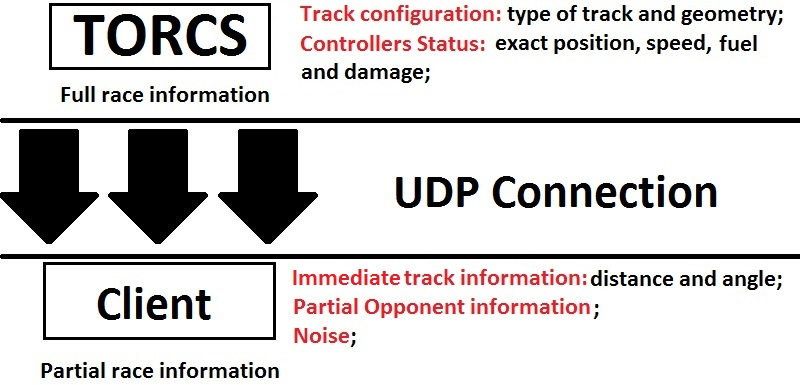
\includegraphics[width=250pt]{Figure1.jpg}
%	\caption{Available data inside TORCS becoming data accessible to the client}
%	\label{Fig:Comm}

% \end{figure}

% Race tracks are categorized into \emph{Road}, \emph{Dirt} and \emph{Oval} inside TORCS. The races from the SCRC take place in track types decided by the organization of the championship, information which is not provided to the participants and that may incorporate maps that are unknown to them. The competition adopts a structure that gathers a \textit{Warm-up} stage, a \textit{Qualifier} stage and a \textit{Final} race. Noise can be introduced in the sensors, option that is present during the actual competition. The complete sensorial input information and all the details concerning the race stages and types are presented at the Simulated Car Racing Championship Competition Software Manual~\cite{SCRC}.

% The reason why TORCS presents itself as a satisfactory AI benchmark, in combination with SCR, is because even	though there are multiple possibilities on how the sensorial input received from the server can be translated into the behavior of the actuators, they can all be compared in a race, which has a robust and steady scoring and evaluational system. In other words, there are many different approaches concerning how to teach the racer encoded by the developers to drive in a racing competition only with the information given by the sensors, and the metric to that issue is the performance on the race itself.



% \section{\textbf{Related Works and State of the Art}} \label{sec:Related}

SCR controllers have been developed using AI techniques, such as neural networks, fuzzy logic, potential fields, and genetic algorithms~\cite{Loiacono:2012:LEA:2212908.2212953}. In the competition, the race track is initially unknown and it several drivers incorporate machine learning procedures to improve their performance~\cite{2009} advantage, which can essentially be \emph{online} or \emph{offline}. Online systems learn by moving about the environment and observing the results while offline ones learn solely by simulating actions within an internal model~\cite{mitchell_1997}.

\emph{Mr. Racer}, which has won the last three championships (2011 to 2013), employs several heuristics and black-box optimization methods in a a modular structure in order to reproduce human-like mechanisms~\cite{MrRacer}, it applies a Covariance Matrix Adaptation Evolution Strategy (CMA-ES), to evolve parameters offline.

In the GECCO leg of the 2013 competition\footnote{\url{http://www.slideshare.net/dloiacono/gecco13scr}}, \emph{AUTOPIA}'s performance stands out. It implements a fuzzy architecture with gear, steering and speed control modules which are optimized offline by a genetic algorithm and an online learning mechanism for landmarking lane exit points to avoid leaving the track~\cite{AUTOPIA}.

Not surprisingly, other participants also use combinations of offline and online learning and modular approaches~\cite{2009,DIEGO,Exp}. Modularity has the clear advantage of independent development and optimization\cite{MrRacer,AUTOPIA2009}, and one of the simplest models for implementing different behaviors is a finite-state machine.

\subsection{Finite-State Machines}%
A FSM is a mathematical model with a finite number of states that can transition from one to another, and a FSM whose output values are determined solely by its current state is a Moore machine~\cite{Ajzerman}. FSMs have been widely used in AI application~\cite{Millington:2006:FSM}, mostly due to its inherent characteristics of flexibility, modularity, and intuitive behavior, among others~\cite{Buckland:2005:AI}.

States are usually implemented with hard-coded rules concerning a specific situation~\cite{Buckland:2005:AI}, which in turn demands small amounts of processor time, and can be easily implemented in different manners. The different driving behaviors can then be coded in parallel with less effort, and easily translated into different states of a FSM. Such approach has successfully been used in SCR~\cite{2009,DIEGO}.

The proper configuration of states and transitions, however, are a more complex problem. Several possible solutions exist, and machine learning techniques can readily be applied.

\subsection{Genetic Algorithms}

GAs are a particular kind of genetic optimization mechanism, inspired by evolutionary algorithms inspired by Darwin's theory of natural selection~\cite{GA}. They are probabilistic search procedures designed to work on large spaces~\cite{goldberg1988}, and have been successful applications in many areas~\cite{GABIO,GAECO,stanley_real-time_2005,pedrycz_genetic_2005}.

GAs work by generating successor solutions by repeatedly mutating and recombining parts of the best currently known solutions, replacing a fraction of the population by offspring~\cite{mitchell_1997}. This is interesting because it works with little information on the problem's domain, the only requirements related specifically to the problem are a representation of a solution for a problem and a function for evaluating it's quality (fitness).

In the context of a self-driving car controller, a solution can be seen as a representation of the driver's parameters and the fitness a measure of its performance, considering speed, safety, fuel consumption, or whatever is the developer's interest. Considering SCR, the usual fitness is the distance driven during the given simulation time~\cite{2009}.

	% \section{\textbf{Related Works}} \label{sec:relworks}
	
		The reason why TORCS presents itself as a satisfactory AI benchmark is because there is an infinity of
		possibilities on how the sensorial input received from the server will be translated into the behaviour of the
		actuators, and they can all be compared in a race, which has a robust and steady scoring system. In other
		words, there are many different approaches concerning how to teach the racer encoded by the developers to
		drive in a racing competition only with the information given by the sensors, and the metric to that issue
		is the performance on the race itself.
		
		By controller, let it be understood that the subject is the programming code that in fact controls the
		car/driver/racer within racing environment. Some examples of awarded controllers and their driving methods
		will be presented in this section. They are what can be called the State of the Art among TORCS, and it is
		very common among them the incorporation of machine learning methods, along with other evolving techniques
		using artificial intelligence. Instinctively, as the nature of the problem comprises evolution by experience,
		learning procedures tend to enhance performance and competitiveness. Essentially, there are two ways of
		evolving controllers: Online Learning and Offline Learning, the first meaning that improvements are achieved
		during the actual race execution time and the latter that it is done before the competition, on the account of
		the developers themselves and with their own resources.
		
\subsection{State of the Art}
		
		The current champion of the SCR Championship is the controller \emph{Mr. Racer}~\cite{MrRacer}, and it has
		proven to be the State of the Art by winning at least the last three competitions that happened. The authors
		of this implementation learn parameters offline through Covariance Matrix Adaptation Evolution Strategy
		(CMA-ES), use regression and low-pass filtering to reduce noise impact, distinguish normal asphalted roads
		from dirt-based ones for behavioral separation and implement an authentic opponent-handling method. Their
		Online Learning consists on the track model selection to categorize into dirt or asphalt, choice of databased
		sets of parameters that best fit the track and the tuning of a target speed for all its corners.
		
		Another renowned controller is \emph{AUTOPIA}~\cite{AUTOPIA}. According to the founders of the
		competition~\cite{SoA} and the authors of \emph{Mr. Racer} themselves, it is a competitive match, with the
		potential to even be the best one available, but since no entries were received from them in a while, their
		means of winning a competition were somewhat restrained. Nevertheless, assessing its performance is
		worthwhile, and its description is the implementation of a modular Fuzzy Architecture, whose division contains
		gear, steering and speed control. Their controller is optimized by means of a genetic algorithm for Online
		Learning, and by means of landmarking the lane exit points for further speed reduction for Offline Learning.\toDo{verificar os termos offline e online}
		
		\toDo{Nós vamos	comparar o nosso piloto com o AUTOPIA? Se sim, devemos dizer isso aqui.}
		
		These and other controller exemplifications served as parameters for the analysis and development of the
		approach presented in this paper. Aspects incorporated and adapted feature modularity, offline learning
		through genetic algorithms, online learning through landmarking and choosing sets of parameters for different
		categories of tracks, etc. \toDo{Adicionar o quê mais fizemos no projeto como pincelada inicial para fazer o
		gancho com a seção Controller Structure.}
	% \section{\textbf{The FSMDriver}} \label{sec:FSM}
	
	Some of the main aspects discussed to outline a controller for TORCS were sufficed by the concept of finite state
	machines (FSM)~\cite{Millington:2006:FSM}, the most important one being the goal of reaching an autonomous driving
	behaviour in a car race.

	According to Mat Buckland in \emph{Programming Game AI By Example}~\cite{Buckland:2005:AI}:
	
	\begin{quotation}
		
		\emph{
			``A finite state machine is a device, or a model of a device, which has a finite number of states it can be in
			at any given time and can operate on input to either make transitions from one state to another or to cause
			an output or action to take place. A finite state machine can only be in one state at any moment in time.''}
		
	\end{quotation}
	
	This architecture was chosen in order to transform the problem of complex driving into smaller problems of
	situations found within the racing environment, and the division performed for the problematic of this work is
	described in the rest of this section.
	
\subsection{Five-state FSM} \label{subsec:FSM5}
	
	Initially, the design of the finite-state machine proposed comprised the following states:
	
	\begin{itemize}

	\item \emph{Straight Line};
	
	\item \emph{Approaching Curve};
	
	\item \emph{Curve};
	
	\item \emph{Out of Track};
	
	\item \emph{Stuck}.

	\end{itemize}
	
	Essentially, for this method, normal behaviour covered \emph{Straight Line}, \emph{Approaching Curve} and
	\emph{Curve}, as the controller was located inside the track boundaries and no recovery actions needed to be
	considered, whereas exception behaviour consisted of \emph{Out of Track} and \emph{Stuck}, situations in which
	such conduct was expected. Here, a consideration needs to be taken into account: the real first model of the
	finite-state machine did not have an \emph{Approaching Curve} state, but, as the interpretations of the demeanour
	concerning the \emph{Straight Line} and the \emph{Curve} were so different from one another, a preparation had to
	be established so as to smoothen the transitions between them.
	
	If the controller was currently in \emph{Straight Line}, it would be expected of him to simply go as fast as he
	could, with no steering changes whatsoever; when in \emph{Approaching Curve} state, he would reposition himself
	in relation to the track and recalibrate his speed in order to make better curves, which is done by steering the
	car towards the direction of the sensor with the biggest read value and braking until a proportionally calculated
	target speed is achieved; or, when in situations of \emph{Curve}, the pilot would stop braking while maintaining
	the steering direction towards the sensor pointing the biggest distance value read - which represents the
	direction of the curve, prepared by the approaching curve state. For the exception states, even though the
	expected deportment is well known, e.g. a stuck controller should maneuver the car out of the current situation
	and proceed to normal race conduct, the implementations vary among developers. The strategy chosen for the
	exception states was used on both proposals as a matter of regularity of comparison, and is explained on the next
	subsection.
	
	One big problem about this way of treating the matter is that the function responsible for choosing which state
	is more appropriate for each situation would more than often be overcharged, and, in some cases, rather different
	sets of parameters received by it would result in the same classification among the states. Thus, in order to
	minimize the dependency of the driving performance in relation to the function in charge of the transition
	between states, a project decision was made to reduce the number of states.
		
\subsection{Three-State FSM} \label{subsec:FSM3}
	
	\toDo{explicar a inicializacao dos vetores de forma gaussiana}
	The very nature of the initial architecture gave rise to the new approach. As mentioned within this very section,
	three of the states were innately part of a common bigger state, thereby \emph{Straight Line},
	\emph{Approaching Curve} and \emph{Curve} summed into \emph{Inside Track}, resulting in the new controller with
	only three states, which were:
	
	\begin{itemize}
		
		\item \emph{Inside Track};
		
		\item \emph{Out of Track};
		
		\item \emph{Stuck}.
		
	\end{itemize}
	
	\emph{Inside Track}, therefore, is how the car, desirably, will spend most part of the time. The controller
	calculates a \emph{target speed} based on how far the car is from the farthest edge of the track, then, it assumes
	a position of increasing the speed until it reaches this velocity while driving towards the sensor with the
	biggest read value. The distance of this method conveys the greater length the car may advance with little or
	sometimes without significant steer changes This state also brakes, if necessary, when approaching turns.
		
	\emph{Out of Track} is when, for any unknown reason, the car is found outside of the track limits. In this case,
	the proper behaviour is to try to return to the lane. In road tracks, the outside track normally has a different
	terrain, sometimes dirt-based, meaning that skidding frequently occurs, and in an effort to avoid this, a control
	system to brake when the car begins skidding above a threshold was implemented.
	
	\emph{Stuck} represents any given situation that the car is unable to progress in the race. This is a delicate
	state, because it presents itself as difficult to identify and also due to its impact to the performance of the
	controller. In order to detect \emph{Stuck} circumstances, the speed of the car is monitored throughout the race,
	during every game tick, if it lingers with a low speed for a determined period, then it is considered stranded,
	or stuck. When detected, this state activates the reverse gear of the car and turns it until its front is
	directed towards the correct axis of the track. The reason why \emph{Stuck} is a sensitive state is because, when
	detected early, might indicate false positive, and when detected late, could lessen the efficiency of the
	controller. Thusly, detecting \textit{Stuck} situations is crucial, and so is handling the car out of them.
	
	Besides the states, there is also a learning module that is called whenever the \emph{Out of Track} state is
	requested. This module records both speed and position from the state of the car in the vicinity of the departure
	from the track, and retaining these information allows the controller to slow down in subsequent laps when
	approaching the critical points highlighted by the learning module. The implementation of this procedure consists
	on replacing the speed recorded for the landmarked position by a slower one on future occurrences, which is done
	by starting to break in these next occasions. For this work, the module described in this paragraph constitutes
	the Online Learning method, concept introduced in Subsection~\ref{subsec:Related}.
	
	In conclusion, each state in this manner of dealing with the process becomes, ideally, an independent problem,
	whose solution can be attacked separately. This way, they can all have individual sets of parameters susceptible
	to improvement, which will be discussed in the next section.
	
\subsection{Search for Parameter Values - Genetic Algorithm} \label{subsec:GA}
	
	Due to the quantity of parameters to be tuned and the defined granularity, the search space becomes enormous and
	renders fundamental the use of a search algorithm, which optimizes the process of finding better configurations
	by being more incisive and saving resources such as computational time and space. In the present study, an
	evolutionary algorithm was chosen for this task.
	
	A genetic algorithm~\cite{GA} is an evolutionary algorithm inspired by nature, in special by the concept of
	evolution through natural selection~\cite{Darwin}, whose main idea is that a set of solutions for a problem can
	be evolved like the population of a generic species in nature. The applications of genetics algorithms are
	present at many areas, extending from control engineering at non-linear system identification to biomedicine
	prosthesis development and even economy to forecast the behavior of agents.\toDo{referencias sobre aplicacoes}
	
	In this context, a viable solution is called an individual and can be represented by a string of parameters. The
	first population is instantiated randomly to its full extent due to the lack of information concerning how to
	effectively evaluate an individual. This population passes through a fitness function that indexes a score to
	each individual, and this function is responsible for assessing how good - or how adapted - the solution that is
	being evaluate is. After evaluating the population separately, a group of individuals is chosen as the parents of
	the next set of solutions, which will compose a new generation; there are countless ways of performing the
	selection of the parents to the new generation of offspring, and this work gave preference to picking the higher
	individuals on the scoring system, what is called Elitism~\cite{ELITISM}. Each pair of parents is submitted to
	crossover in order to generate two offspring solutions, and in the end of the process each offspring may present
	mutation - everything according to predefined rates. For this work, the crossover takes place in 95\% of the
	reproduction, while the mutation rate assumes the rate of 1\%~\cite{RATES}.
	
	For the Five-state FSM, 22 parameters required adjustment, which originated, in different quantities, from each
	state separately and also the \emph{transition} function, as follows:
	
	\begin{itemize}
		
		\item \emph{Approach Curve} has 4 parameters;
		
		\item \emph{Transition Function} has 3 parameters;
		
		\item \emph{Straight Line} has 4 parameters;
		
		\item \emph{Out of Track} has 7 parameters;
		
		\item \emph{Stuck} has 4 parameters.
		
	\end{itemize}
	
	However, for the Three-state FSM, only 19 parameters demanded adjustment, which are divided as follows:
	
	\begin{itemize}
		
		\item \emph{Inside Track} has 8 parameters;
		
		\item \emph{Out of Track} has 7 parameters;
		
		\item \emph{Stuck} has 4 parameters.
		
	\end{itemize}
	
	Theoretically, as the search space for the latter case is smaller, finding a better controller was expected to
	happen first for it, but only by effectively testing both architectures could such a result be achieved. The
	source codes for both models presented in this section are available at the \emph{GitHub} repository provided in
	the references~\cite{GitHub}.
	
	% \section{Experimental Results} \label{sec:Experiments}

	A veil was put over the Five-state FSM from the very beginning of the experimentation phase, which was its great dependency towards the transition function. Early superficial evaluations of the performance of this first model indicated an overcharge concerning this function, which was verified by considerable changes in behaviour derived from adjustments in its parameters. For that reason, a second model with less states - the Three-state FSM - was designed regarding this characteristic and releasing part of the performance burden from the transition function, and the results from the comparison of these architectures are described and analyzed in the succeeding subsections.

\subsection{Methodology} \label{subsec:Methodology}

	Once the models - and which of their parameters required tuning - had been defined, the genetic algorithm was applied to each approach separately, in order to adjust their configurations for superior and competitive status. At the same time, the goal was to find general and versatile controllers with good results for any track and specific ones that were fittest to race in various tracks: road, dirt and oval alike. Therefore, due to the differences observed in the parameters of controllers evolved on dirt and road tracks, the evolution process took place separately for those two kinds of environments, which produced two contrasting sets of enhanced values for each model.
	
	The \emph{metric} chosen to evaluate the generated controllers was the combined sum of the distance raced by the car alone in the first 10 000 game cycles - also called \emph{game tics} - in a list of mixed tracks. This value will henceforth be called the \emph{fitness} of the controller, as it was used to determine whether he would remain in the evolution process.
	
	The experiments concerning Oval Tracks would repeatedly provide inconclusive results, so they were neglected in this evaluation process. Thus, in order to find the best set of parameters for a general track, the two finite-state states were evolved in three different sets of tracks, one with 4 Dirt Tracks, one with 4 Road Tracks and another with the 4 of each type. The evolution process for each set of tracks consisted on 600 generations of 30 individuals and culminated in one controller; in other words, at the end of the experiments, there were six evolved controllers, one specific for Road Tracks for each model, one specific for Dirt Tracks for each model, and also one evolved in a mixed manner for each model. Additionally, as the \emph{Stuck State} is only triggered in very specific situations, it was not evolved with the controller and its parameters were hand tuned.
	
	Pursuing an unbiased choice of parameters, the Online Learning module described in Subsection~\ref{subsec:FSM3} was turned off during the evolution progress as it seizes the responsibility for the behaviour of the car for itself during the race and could interfere with natural selection. The validation then occurred through testing the six produced pilots in a predefined set of tracks different from those in which they were evolved, avoiding the evidence of too track-limited parameters. On behalf of comparison, the results from the AUTOPIA controller were incorporated in the analysis, since it can be considered the State of the Art, displaying one of the best performances for the SCR Championship, and should provide satisfactory basis for appraisal.

	The four Road Tracks used in the evolution process were chosen from the TORCS standard track set, which are \emph{Spring}, the longest track available on TORCS with more curves than any other track, \emph{Wheel 2}, the most difficult track with sharp and hard curves, \emph{E-Track 3}, a fast track with turns that put to test the dexterity of the controller, and \emph{Forza}, a track considered to be raced fast and whose curve pattern is usually found in others tracks. Also four Dirt Tracks were selected to be used in evolution, which were \emph{Dirt2}, \emph{Mixed1}, \emph{Mixed2}, \emph{Dirt6}. \emph{Dirt2} is a difficult track with close curves, while \emph{Mixed1} is an easy one with few curves, also, \emph{Mixed2} has many turns with medium difficulty, and \emph{Dirt6} present hard curves.
	
	Once the evolution process was finished, the six resultant controllers were tested in the evaluation set of tracks, different from those where they were evolved. Three Road Tracks were picked to evaluate the controllers, they are also available on TORCS and were used both in the competitions of 2008 and to evaluate the \emph{AUTOPIA} controller~\cite{AUTOPIA2009}. \emph{Street-1} and \emph{D-Speedway} were used at the \emph{IEEE World Congress on Computational Intelligence}; and \emph{CG Speedway 1} was used at the \emph{Computational Intelligence and Games Symposium - CIG}. This set also contained three Dirt Tracks, which were \emph{Dirt1}, \emph{Dirt3}, \emph{Dirt4}. \emph{Dirt1} has smooth curves and allows the controller to perform in high speed, while \emph{Dirt3} is an easy one with few curves, also, \emph{Dirt4} has many turns with medium difficulty and is the longest Dirt Track available.
	  
	
\subsection{Results} \label{subsec:Results}
	
	It is important to mention that before each result displayed in that section a warm-up stage was held for 5 laps in each track.
	
	The controllers were submitted to a set of evaluation races and the distances they covered in 10 000 game tics inside each of those races were joined in Table~\ref{tbl:dist covered}. This table also displays how the evolved controllers performed in comparison to the AUTOPIA controller.
	
	In order to have a more in-depth comparison, Table~\ref{tbl:time raced} was assembled to display the time elapsed during 10 laps for each of the previous tracks tested. The \textit{Berniw Hist4} bot provided by the TORCS distribution was also used in this test phase even though it uses a different car from those allowed in the SCRC~\cite{2009} and has a low performance compared to the others bots provided. AUTOPIA also uses this bot for comparison~\cite{AUTOPIA}.
	
	\begin{table*}[t]
	\renewcommand{\arraystretch}{1.3}
	\caption{Distance covered in meters racing alone for 10 000 game tics}
	\label{tbl:dist covered}
	\centering
	\begin{tabular}{c||c||c||c||c||c||c}
	\hline
	\bfseries Driver & \bfseries Street-1 & \bfseries D-speedway & \bfseries CG-speedway & \bfseries Dirt-1 & \bfseries Dirt-3 & \bfseries Dirt-4 \\ 
	\hline	
	\hline FSM3(road) & \textbf{7925.6} & 13196.5 & 8745.49 & 3978.01 & 3451.26 & 6757.83 \\
	\hline FSM3(dirt) & 2149.77	& 2450.84 & 1951.93	& 3525.84 & 4905.58 & 5590.78 \\
	\hline FSM3(mixed) & 7219.28 & 12772.4 & 8126.12 & \textbf{4386.64} & \textbf{5481.15} & \textbf{6939.83} \\
	\hline FSM5(road) & 3822.76 & 3427.11 & 4114.66	& 2145.49 &	2205.97 & 3260.19 \\
	\hline FSM5(dirt) & 1267.83 & 2936.82 &	4114.66 & 1072.92 &	2205.82 & 3260.33 \\
	\hline FSM5(mixed) & 3822.99 & 3427.06 & 4114.8 & 2145.75 &	2205.83 & 3260.31 \\
	\hline AUTOPIA & 7091.8 & \textbf{15612.3} & \textbf{8970.4} & * & * & * \\
	\hline 
	\end{tabular} 
	\end{table*}

	
	\begin{table*}[t]
	\renewcommand{\arraystretch}{1.3}
	\caption{Time elapsed in seconds racing alone for 10 laps}
	\label{tbl:time raced}
	\centering
	\begin{tabular}{c||c||c||c||c||c||c}
	\hline
	\bfseries Driver & \bfseries Street-1 & \bfseries D-speedway & \bfseries CG-speedway & \bfseries Dirt-1 & \bfseries Dirt-3 & \bfseries Dirt-4 \\ 
	\hline
		\hline FSM3(road) & \textbf{1086.3} & 607.4 & \textbf{495.0} & \textdagger & 1150.1 & 1756.4 \\
	\hline FSM3(dirt) & \textdagger & 840.0 & 1274.8 & 597.3 & 1089.4 & 1307.5 \\
	\hline FSM3(mixed) & 1216.50 & \textbf{572.60} & 613.77& 530.0 & 842.9 & 1005.9 \\
	\hline FSM5(road) & \textdagger & \textdagger & 816.6 & \textdagger & \textdagger & \textdagger \\
	\hline FSM5(dirt) & \textdagger & \textdagger & \textdagger & \textdagger &	\textdagger & \textdagger \\
	\hline FSM5(mixed) & \textdagger & \textdagger & \textdagger & \textdagger & \textdagger & \textdagger \\
	\hline Berniw Hist4 Bot & 1143.77 & 656.24 & 605.76 & 460.95 & 872.97 & 1127.45 \\
	\hline AUTOPIA & * & * & * & \textbf{339.3} & \textbf{742.4} & \textbf{796.5} \\
	\hline 
	\end{tabular} 
	\end{table*}
	
	It is important to mention that the bots have a full view of the track format and do not use the sensors provided by SCR. Instead, they have directly access to all the information necessary to race, which gives them some advantage over the controllers developed for the TORCS environment, such as the ones described in this paper, which receive only the information that comes from sensors and in addition have to interpret them in order to abstract how the track really is. 
	
\subsection{Analysis} \label{subsec:Analysis}
	
	The best pilots from each race evaluated by Tables~\ref{tbl:dist covered} and~\ref{tbl:time raced} were highlighted in bold. Both sets of experimental results shown at these tables were selected in order to match previous tests performed by the AUTOPIA controller. In 2009, the authors of AUTOPIA~\cite{AUTOPIA2009} evaluated it through racing for a predefined time period and computing the total distance reached, and these results were incorporated in Table~\ref{tbl:dist covered} for comparison. Differently, in 2012, this controller~\cite{AUTOPIA} was assessed by racing alone during 10 laps and calculating the time elapsed to do so, and these results were also incorporated in the evaluation process of this paper and are displayed in Table~\ref{tbl:time raced}. The tracks that are not present in either of the tests executed by AUTOPIA were validated only between the approaches proposed by this paper, which was informed in Tables~\ref{tbl:dist covered} and~\ref{tbl:time raced} through the ``*'' symbol, meaning that AUTOPIA had no results for that race in particular.
	
	For a wider analysis not only the numeric results were taken into account in this section but also observations made in the graphic mode provided by the TORCS distribution.
\subsubsection{Comparing the Controllers Proposed} \label{subsubsec:CompControllers}
	
	The overall comparison between the two approaches presented favored the Three-State FSM, on account of the considerably superior results it produced in all the tracks tested. The Five-State FSM presents a very complex transition function that takes into account the variance of the sensorial input to decide if the car is in a straight line, approaching a turn or in a turn. On the other hand, the Three-State FSM has only a single state for handling normal driving situations and it is very easy to say if the controller is inside or outside the track only by checking the track sensor. This contrast in behavior is then interpreted to be the reason of the overwhelming difference in performance, the complexity of the transition function, which supports the initial hypothesis of the evaluation. Due to this attribute, the Five-State FSM undergoes a lot of damage in its car, which can be noted in Table~\ref{tbl:time raced} where all the ``\textdagger'' symbols represent individuals that did not finish the race for the reason of reaching the maximum damage permitted.
	
	Because the Three-State FSM demonstrated better results than the other approach proposed, it was elected to be subject of analysis on the evaluation process. As expected, the controller evolved only on Road Tracks was the fastest one. These tracks provide an environment susceptible to high speeds, since its curves are smoother and the friction experienced by the car is higher than the ones from Dirt Tracks. These factors, when combined, allow the controller to race without having to steer too abruptly and to brake without losing control while racing in Road Tracks. Consequently, as the friction increases, steering becomes more accurate in road tracks, practically eliminating critical skidding. Therefore, the result from this end of the evolution process was an aggressive driver with high base-speed.
	
	Dirt Tracks provide a more difficult environment for the pilot to fit in. Sudden braking in tracks of this type often results in unwanted behavior, skidding is noticeably more common then. The driver evolved in this end of the evolution process tends to drive in a low speed so it can keep itself inside the boundaries of the track. Speed driving results in higher damage outcomes and even in the total loss of the car in critical situations. The result obtained was a very careful driver with a low base-speed, and an early brake policy - the car starting to brake far before the turn. This passive driving pattern obtained the smallest distance covered both for the Three-State and the Five-State FSMs.
	
	The driver evolved in a mixed set of tracks combines characteristics from both of them. It drives in a reasonable speed comparing to the first one, but also has the preventive brake policy from the second one. This last end of the evolution process achieved better results than the dirt-evolved behavior in all the tracks tested and outperformed the road-evolved one in every single dirt track. From this information gathered, it was inferred that the controller evolved in mixed tracks tries to reach higher speeds even though this means leaving the track in some turns, mostly because the time spent trying to get back to the racing lane is compensated by the speed of the car. The aggressive behavior inherited from the road-evolved end of the evolution makes this latest controller receive ample damage when leaving the track, and also causes it to hit walls, which resulted in the premature ending of some of the tested races, due to reaching the maximum acceptable damage.
	
\subsubsection{Comparing the Three-State FSM to AUTOPIA} \label{subsubsec:CompAUTOPIA}

	Once the Three-State FSM was demonstrated to be more suitable to competitive environments due to its superior performance regarding the Five-State FSM, it was compared to the renowned controller AUTOPIA. Using the distance covered after racing alone in Road Tracks for 10 000 game tics as metric, the Three-State FSMs evolved in Road Tracks and in mixed tracks were able to overcome AUTOPIA in 1 of the 3 tracks tested, as displayed in the bold values in Table~\ref{tbl:dist covered}. The road-evolved Three-State FSM was the controller that got closer to this State of the Art approach using the ``distance raced'', which comes to endorse the assumption of it being a competitive proposal.
	
	However, while racing alone for 10 laps and computing the time elapsed as metric, AUTOPIA outperformed every controller proposed, just as can be seen in Table~\ref{tbl:time raced}. Even though the Three-State controller with Road evolved parameters outperformed AUTOPIA in the first 10 000 tics it was not capable of maintaining the advantage in longer races. As the road evolved pilot presents a more aggressive behavior even though it means taking more damage it has a gain in performance for the early stages of the race. Although when racing for more than a couple laps the controller becomes more careful after each lap reducing it speed to maintain itself inside the track.
	
	The online learning module plays a crucial role in the overall controller's performance as it prevents unwanted situations to repeat, for example leaving the track. Although this strong dependence might result in performance loss as the controller will gradually reduces it speed after each lap in those points where it leaves the track. More accurate actuators control may reduce the dependence of this module and therefore improves performance.
	
	These results can be used to infer that the Five-State and the Three-State FSMs have a great deal of improvement to achieve when it comes to endurance. The Five-State FSM received total loss and did not complete almost every test performed, ending only one race using this metric. The Three-State FSM, on the other hand, completed practically all the tracks, but did not surpass AUTOPIA in either of them. In order to enhance the endurance feature in the controllers proposed, more robust behavior concerning situations in which the car might crash must be taken into account.	
	
	
	% \section{Conclusions} \label{sec:Conclusions}

	This paper proposed two approaches developed to control a car during a race in a simulated computational environment, the game platform TORCS. The models of both of these controllers were described, explained, enhanced by means of a genetic algorithm, compared and then tested together with a State of the Art controller - AUTOPIA. It was implied before the testing phase that a finite state machine too burdened in the process of transition between states might lose performance, which was corroborated by the experimental results of the comparison of the two models detailed.
		
\subsection{Conclusions} \label{subsec:Conclusions}

	The finite state machine with less states achieved a superior overall performance in the tests carried out, in relation to the one with more states. The simplifications fashioned in the transition function of the former were inferred to be the reason for this improvement, along with its intricate relation with the number of parameters that were target of fine tuning in the evaluation and validation process.
	
	The evolution procedure adopted concerning the controllers culminated in three characteristic behaviors. The controller evolved on road tracks became a fast driver, whose hastiness resulted in a careless attitude in general; in other words, it was only good for races in road tracks. The one evolved on dirt tracks turned out to be too careful in contrast, limitedly determining its speeds and, in efficiency terms, inferior. The controller evolved on a mixed set of tracks inherited characteristics from both the previous ones, becoming swift but not too hasty, prudent but not too slow. The latter surpassed the performance of the dirt-evolved drivers even on dirt tracks, and did not lose by far on road tracks in comparison to drivers evolved solely in them.
	
	In terms of speed, the Three-State FSM was able to overcome AUTOPIA in one of the three tracks used to validate the drivers using the distance covered in 10 000 game tics as metric. However, in comparison to the same controller, using the time elapsed to race 10 laps as metric instead, the experimental results provided an insight on the lack of endurance that the finite state machine drivers proposed possess.
	
	To sum up, the interpretation of the global results from the experiments performed gives margin to declare that finite state machines are a reliable technique to implement artificial intelligences, at least for computer games such as simulated races. They provide the possibility of parallel development and also enable parameter tuning in separate fronts, due to the independence and abstraction between the behaviors from each state. Finite state machines also represent a valuable tool for describing an operation model for a process, simplifying and gathering possible situations it might present into straightforward categories of accessible understanding.

\subsection{Future Works} \label{subsec:Future}
	
	One characteristic that has been marked as a deficiency in the controllers presented in this paper is the lack of endurance. In order to prevent this from affecting the general performance of the controllers developed, more robust techniques must be integrated into their model. Ways of treating this matter range from harsher brake policies to drive planning intensification, which are already being taken into account for future proposals.
		
	Another important task to be accomplished is the opponent treatment in real-time races. Routines to reduce collisions, i.e., avoiding being overtaken and also being concerned about overtaking the opponents is a fundamental issue. Ignoring adjacent cars usually causes the driver to face unexpected collisions, ending up stuck, considering a worst case scenario. Many of the renowned developers for TORCS already incorporate such treatment in their controllers, and neglecting this necessity renders any driver less robust to unexpected race events, and also reduces its performance.
	
	

	%\section*{Acknowledgements}

	\bibliographystyle{sbgames}
	\bibliography{Bibliography}

\end{document}
